% REMEMBER: Write the thesis from the view of the reader. How would I like to READ the thesis?
% WHY -> WHAT -> HOW structure

% 6th, 7th grade

\chapter{Evaluation}%
\label{cha:evaluation}

In this chapter, Whisker will be evaluated.
We will conduct three experiments to answer the following research questions.

{
    \parspace

    \centering
    \begin{minipage}{.9\textwidth}
        \textbf{RQ1: Can results of automated testing be accurate enough to aid in grading Scratch assignments?}
        \parspace

        \noindent \textbf{RQ2: Is automated test input generation a viable method to control Scratch programs for testing purposes?}
        \parspace

        \noindent \textbf{RQ3: Does the testing process slow down the program under test?}
    \end{minipage}

    \parspace
}


\noindent In the first experiment we will execute three different test suites on a set of Scratch projects,
then examine the test results to determine their accuracy.
For the second experiment, we will execute automated input generation on a variety of projects,
and measure the achieved statement coverage to find out how much of ordinary Scratch programs
can be reached by automatically generated input.
Finally, in the third experiment we will measure execution times
to check if the testing process slows down the program under test.
\parspace


Initially, Section 4.1 describes the evaluation method used in this work.
Afterwards, the strategy used for comparing both approaches is explained in Section
4.2. Section 4.3 describes which subjects are used for the evaluation and why, before
the actual results are shown in Section 4.5. Finally, Section 4.6 discusses the results und
points out possible threats to validity.
4.1
Method Selection
When performing empirical evaluations, a variety of possibilities to measure the quality




\section{Experimental Setup}
\label{sec:experimental_setup}

\subsection{Testing Environment}

We executed test suites on several Scratch programs through Whisker's web interface.
The software and hardware we used are listed in Figure~\ref{tab:evaluation_setup}.
All test executions were performed on the same machine.
For two parts of the evaluation,
specifically to measure execution time and to measure coverage over time,
we used slightly modified versions of Whisker as well as its GUI.

\begin{table}[htpb]
    \centering
    \scriptsize \tt
    \begin{tabular}{ll}
        \toprule
        Whisker     & Whisker 1.0 \\
        Scratch VM  & Scratch VM 0.2.0-prerelease.20181005173109 \\
        Web Browser & Chrome 70.0.3538.110 (64-Bit) \\
        JavaScript  & V8 7.0.276.40 \\
        OS          & Windows 8.1 Version 6.3 (Build 9600) \\
        CPU         & Intel Core i5 4670 (4 x  3.40 GHz) \\
        GPU         & Nvidia GeForce GTX 1080 \\
        RAM         & 8GB DDR3-1600 \\
        \bottomrule
    \end{tabular}
    \caption{Software and hardware used for evaluation}
    \label{tab:evaluation_setup}
\end{table}

\subsection{Projects Under Test}

This section will list the Scratch projects,
which we used to evaluate Whisker,
and explain, why these projects were chosen.

\subsubsection{(P1) Catching Game}

The first set of Scratch projects consists of 41 student implementations of a simple catching game.
The projects originate from a voluntary Scratch course for 6th and 7th grade students.
In this course, students were introduced to Scratch through several small exercises,
% familiarized themselves with Scratch
building up to the final and most complex exercise to develop the aforementioned catching game.
Students were given a project as a template to fill with their implementation.
\parspace

In this game, apples and bananas periodically fall from the top of the screen.
The player earns points by catching these fruits with a bowl at the bottom of the screen,
which is controlled with the left and right arrow keys.
The game ends when 30 seconds have passed or if an apple touches the ground (a game over).
A screenshot of the sample implementation of this program can be seen in Figure~\ref{fig:screenshot_of_the_sample_implementation}.
Additionally, a summary of the full program specification from the assignment may be found in Table~\ref{tab:project_specification}.
\mnote{TODO: assignment in the appendix?}
\parspace

\begin{figure}[htpb]
    \centering
    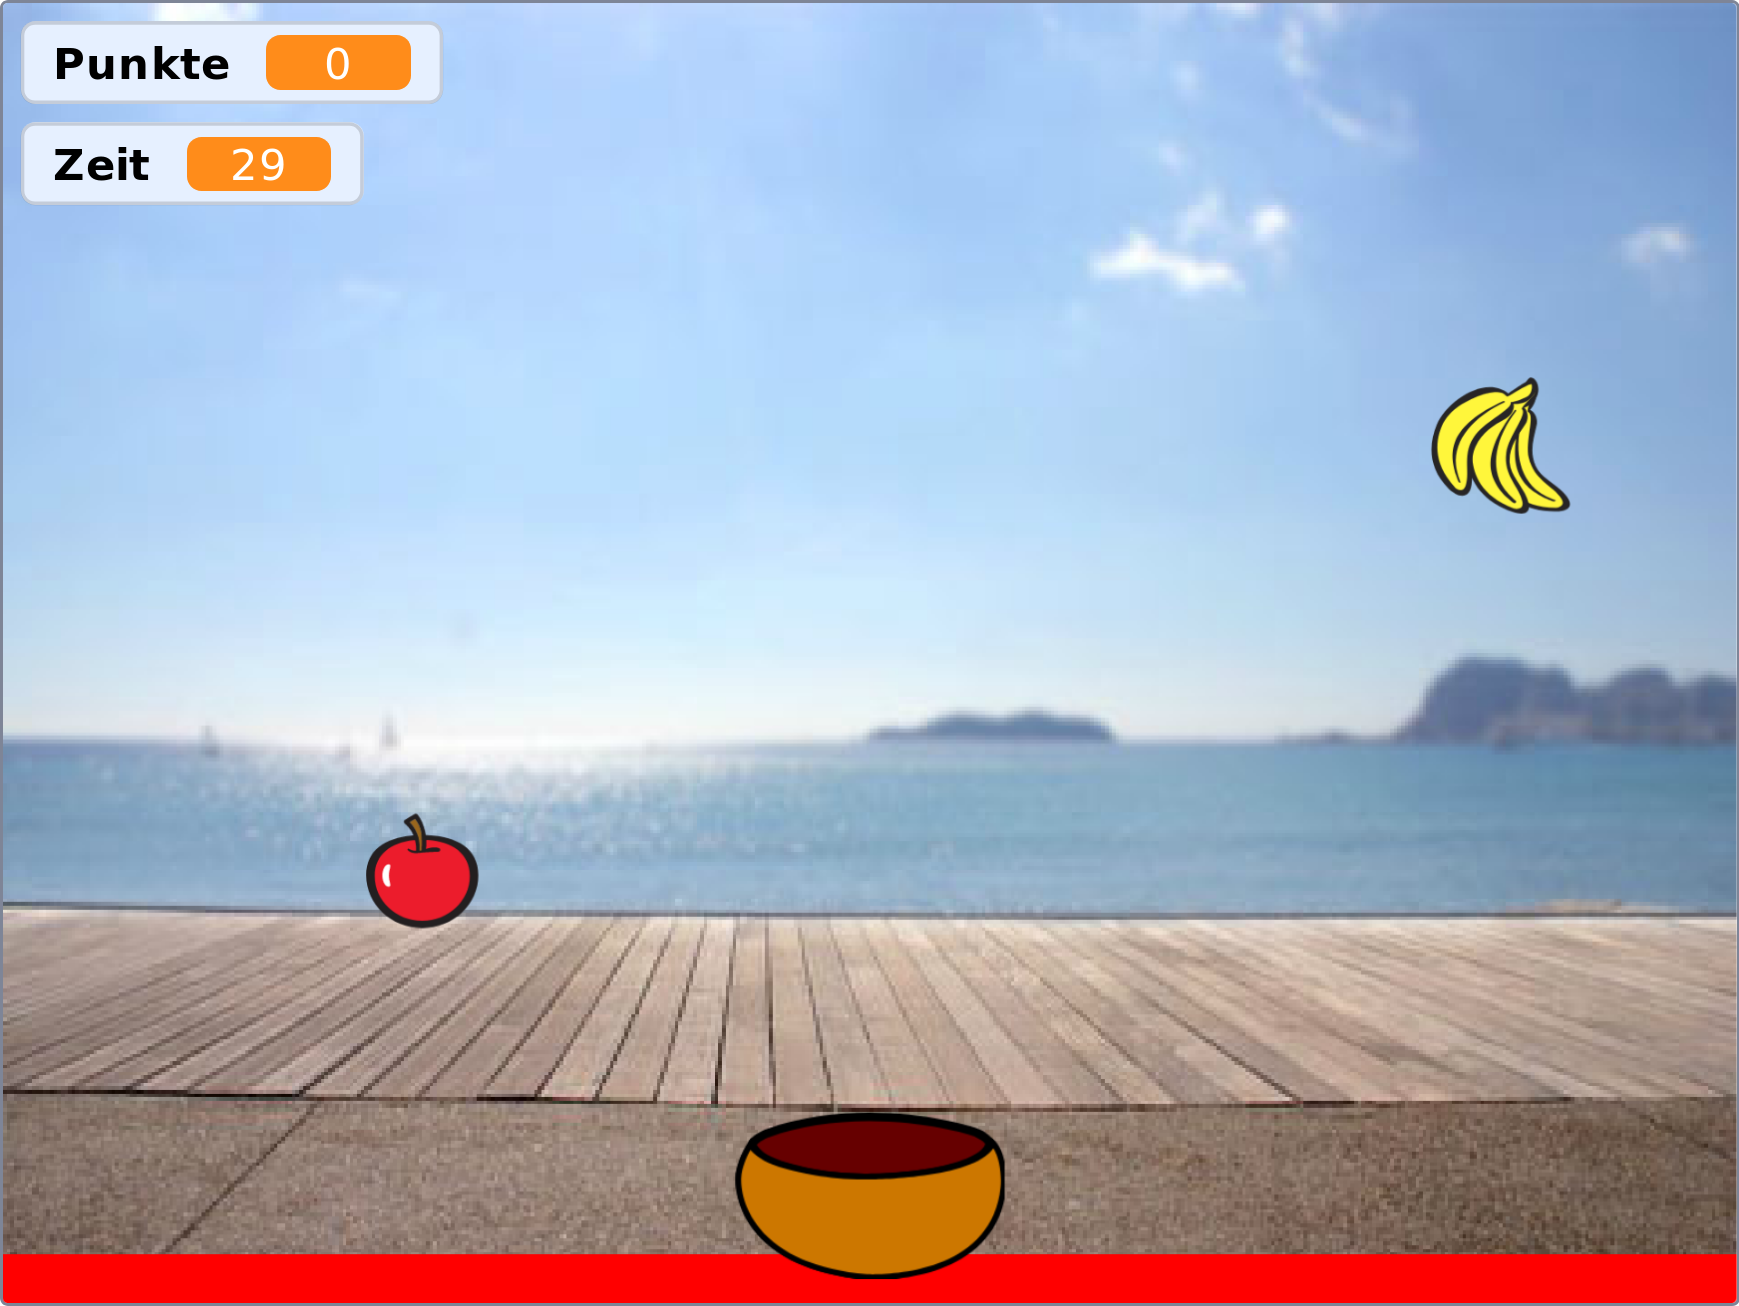
\includegraphics[width=0.35\textwidth]{scratch-stage}
    \caption{Screenshot of the sample implementation}
    \label{fig:screenshot_of_the_sample_implementation}
\end{figure}

We will execute various test suites on these programs to analyze their results.
The Scratch projects in this set were manually evaluated and scored for the students course.
This enables us to determine the quality of our test results by using the manually assigned scores as ground truth,
and comparing the results of automated testing to them.
\parspace

The projects are suitable for this evaluation because of two reasons.
Firstly, the task description specifies the program well, which enables us to write automated tests according to the specification.
Secondly, the student solutions are of varying degrees of quality,
which is desirable, so automated tests produce a range of different outcomes.
% Some of the projects implement the game almost perfectly,
% while many contain common errors, and some don't work correctly at all.
However, testing these projects has also revealed some challenges.
For one thing, these projects were never meant to be subject to automated testing.
Therefore, some details, mainly the usage of clones,
are not part of the task specification, which complicates testing,
since tests have to consider multiple options.
Additionally, the game over state, that the program enters,
when an apple touches the ground, also makes automated testing more difficult.
\parspace

Since the students didn't write the programs with automated testing in mind,
some of the projects were unusable for our evaluation for various reasons, so we excluded them from the statistics.
Table~\ref{tab:excluded_projects} shows the excluded projects together with the reasons for excluding them.
The projects are named K6\_S01 through K6\_S33 for 6th grade student solutions
and K7\_S02 through K7\_S27 for 7th grade student solutions respectively (with many numbers being skipped).
Most of the excluded projects were found by analyzing the test reports and the coverage of our test suite,
while two of them were detected manually from a discrepancy between our test results and the manual scoring,
which we will compare our results to later.

% === Excluded Projects
% - Some of the projects were excluded from the evaluation
% - Because they where problematic to automated testing in some way
%     - Tests select sprites and variables by name, and some projects changed the names of sprites and variables
%         - Detected by searching the test reports: ''grep''
%     - Some projects used a different mechanism than the green flag to start their program
%         - Since this is not specified, tests can not start the program
%         - Detected by zero statement coverage
%     - Some Projects didn't work properly because of missing initialization
%         - Go game over on startup
%         - One project work if green flag is pressed multiple times
%         - One project only worked if the sprites were manually dragged to a different position

\begin{table}[htpb]
    \centering
    \scriptsize
    \begin{tabular}{lp{10.5cm}}
        \toprule
        Project & Reason                                                                          \\
        \midrule
        \multicolumn{2}{l}{\textbf{Detected through test reports}}                                \\
        K6\_S12 & Deleted variable from template: ''Zeit''                                        \\
        K6\_S17 & Renamed variable from template: ''Punkte'' to ''Bunkte''                        \\
        K7\_S24 & Deleted variable from template: ''Zeit''                                        \\
        K7\_S27 & Renamed sprite from template: ''Bowl'' to ''Figur2''                            \\
        K7\_S07 & Resets all sprite positions when the "a" key is pressed.
                  Problematic, because automated test input generation will press the "a" key     \\[1.4\bigskipamount]

        \multicolumn{2}{l}{\textbf{Detected through zero statement coverage}}                     \\
        K6\_S01 & Starts on up arrow key press instead of green flag                              \\
        K6\_S06 & Wrong scratch project file (scored 30 points in manual rating but has no code)  \\
        K6\_S14 & Starts on space key press instead of green flag                                 \\[\medskipamount]

        \multicolumn{2}{l}{\textbf{Detected manually}}                                            \\
        K6\_S20 & Green flag has to be pressed twice to make it work properly                     \\
        K7\_S18 & Sprites have to be repositioned manually in the editor to make it work properly \\
        \bottomrule
    \end{tabular}
    \caption{Excluded projects together with the reason to exclude them}
    \label{tab:excluded_projects}
\end{table}

\subsubsection{(P2) Code Club Projects}

The second set of Scratch projects consists of sample solutions to 24 of Code Club's~\cite{codeclub} Scratch exercises.
Code Club offers free coding projects and step by step guide for programming beginners.
For each project, a sample solution is provided by a volunteer.
\parspace

\mnote{Add a table which lists the projects?}
We use these projects to evaluate Whisker's automated test input generation by measuring its achieved coverage.
The projects work well for this task since they implement a variety of different programs with different input methods.
We chose the sample solutions of the exercises since measuring coverage on working implementation will yield better results.
Broken implementations may be more likely to have unreachable code,
because some code might depend on a feature, that is not implemented correctly.

\subsection{Test Suites}

The set of catching game projects (P1) will be tested with three different test suites in order to analyze the quality of test results.
Table~\ref{tab:project_specification} lists which part of the specification is covered by each test suite.
Additionally, the number of tests or constraints and the size of the test suite, measured in lines of code (LOC),
can be found in Table~\ref{tab:test_suite_statistics}.

\begin{table}[htpb]
    \centering
    \scriptsize
    \begin{tabular}{rlrlr}
        \toprule
        Test Suite & Type       & \texttt{\#}Tests / \texttt{\#}Constraints & LOC \\
        \midrule
        T1         & Normal     & 28 Tests                                  & 852 \\
        T2         & Constraint & 20 Constraints                            & 515 \\
        T3         & Constraint & 18 Constraints                            & 539 \\
        \bottomrule
    \end{tabular}

    \caption{Number of tests and LOC per test suite}
    \label{tab:test_suite_statistics}
\end{table}

\begin{table}[htpb]
    \centering
    \scriptsize
    \begin{tabular}{rl|cr|cr|cr}
        \toprule
        \texttt{\#} & Specification                                                    & \multicolumn{6}{c}{Covered? (\xmark/\cmark), Test number}                     \\
                                                                                      && \multicolumn{2}{l|}{T1} & \multicolumn{2}{l|}{T2} & \multicolumn{2}{l}{T3}    \\
        \midrule
           & \textbf{Initialization} &&&&&&\\
         1 & Timer starts at 30 seconds                                                & \cmark & 1  & \xmark                    &    & \xmark                    &    \\
         2 & Bowl starts at $X = 0$ / $Y = -145$                                       & \cmark & 2  & \xmark                    &    & \xmark                    &    \\
         3 & Fruits have a size of 50\%                                                & \cmark & 3  & \cmark                    & 1  & \cmark                    & 1  \\[\medskipamount]
           & \textbf{Bowl Movement} &&&&&&\\
         4 & Bowl moves left/right when corresponding arrow key is pressed             & \cmark & 4  & \cmark                    & 2  & \cmark                    & 2  \\
         5 & Bowl can only move horizontally with a speed of 10                        & \cmark & 5  & \cmark                    & 3  & \cmark                    & 3  \\[\medskipamount]
           & \textbf{Fruit Falling} &&&&&&\\
         6 & Apples fall down                                                          & \cmark & 6  & \textasteriskcentered$^1$ &    & \textasteriskcentered$^1$ &    \\
         7 & Apples fall in a straight line with a speed of -5                         & \cmark & 7  & \cmark                    & 4  & \cmark                    & 4  \\
         8 & Bananas fall down                                                         & \cmark & 8  & \textasteriskcentered$^2$ &    & \textasteriskcentered$^2$ &    \\
         9 & Bananas fall in a straight line with a speed of -7                        & \cmark & 9  & \cmark                    & 5  & \cmark                    & 5  \\[\medskipamount]
           & \textbf{Fruit Spawn} &&&&&&\\
        10 & Apples spawn again at the top of the screen after touching the bowl       & \cmark & 10 & \textasteriskcentered$^3$ &    & \textasteriskcentered$^3$ &    \\
        11 & Apples spawn at random $X$ position                                       & \cmark & 11 & \cmark                    & 6  & \cmark                    & 6  \\
        12 & Apples spawn at $Y = 170$                                                 & \cmark & 12 & \cmark                    & 7  & \cmark                    & 7  \\
        13 & Bananas spawn again at the top of the screen after touching the bowl      & \cmark & 13 & \textasteriskcentered$^4$ &    & \textasteriskcentered$^4$ &    \\
        14 & Bananas spawn at random $X$ position                                      & \cmark & 14 & \cmark                    & 8  & \cmark                    & 8  \\
        15 & Bananas spawn at $Y = 170$                                                & \cmark & 15 & \cmark                    & 9  & \cmark                    & 9  \\
        16 & Only one apple must fall down at a time                                   & \cmark & 16 & \cmark                    & 10 & \cmark                    & 10 \\
        17 & Only one banana must fall down at a time                                  & \cmark & 17 & \cmark                    & 11 & \cmark                    & 11 \\
        18 & Banana must wait for a second before falling down in the beginning        & \cmark & 18 & \xmark                    &    & \xmark                    &    \\
        19 & Banana must wait for a second before falling down after displaying ''-8'' & \cmark & 19 & \xmark                    &    & \xmark                    &    \\[\medskipamount]
           & \textbf{Fruit Interaction} &&&&&&\\
        20 & Apple gives 5 points when it touches the bowl                             & \cmark & 20 & \cmark                    & 12 & \cmark                    & 12 \\
        21 & Game over when the apple touches the ground                               & \cmark & 21 & \textasteriskcentered$^5$ & 13 & \cmark                    & 13 \\
        22 & Apple displays ''Game Over!'' message when it touches the ground          & \cmark & 22 & \textasteriskcentered$^5$ & 14 & \cmark                    & 14 \\
        23 & Banana gives 8 points when it touches the bowl                            & \cmark & 23 & \cmark                    & 15 & \cmark                    & 15 \\
        24 & Banana subtracts 8 points when it touches the ground                      & \cmark & 24 & \cmark                    & 16 & \cmark                    & 16 \\
        25 & Banana displays ''-8'' message when it touches the ground                 & \cmark & 25 & \cmark                    & 17 & \cmark                    & 17 \\[\medskipamount]
           & \textbf{Timer} &&&&&&\\
        26 & Timer ticks down                                                          & \cmark & 26 & \cmark                    & 18 & \cmark                    & 18 \\
        27 & Game stops when timer reaches 0                                           & \cmark & 27 & \cmark                    & 19 & \xmark                    &    \\
        28 & Bowl must display ''Ende!'' message when timer reaches 0                  & \cmark & 28 & \cmark                    & 20 & \xmark                    &    \\
        \bottomrule \\
        \multicolumn{1}{r}{\textasteriskcentered$^1$} & \multicolumn{1}{l}{Not covered directly, because indirectly covered by (7)        } \\
        \multicolumn{1}{r}{\textasteriskcentered$^2$} & \multicolumn{1}{l}{Not covered directly, because indirectly covered by (9)        } \\
        \multicolumn{1}{r}{\textasteriskcentered$^3$} & \multicolumn{1}{l}{Not covered directly, because indirectly covered by (11), (12) } \\
        \multicolumn{1}{r}{\textasteriskcentered$^4$} & \multicolumn{1}{l}{Not covered directly, because indirectly covered by (14), (15) } \\
        \multicolumn{1}{r}{\textasteriskcentered$^5$} & \multicolumn{1}{l}{Covered, but game over through apple not expected to happen    } \\
    \end{tabular}

    \caption{Project specifications and their coverage by the test suites}
    \label{tab:project_specification}
\end{table}

\subsubsection{(T1) Normal Test Suite}

This test suite follows an ordinary testing approach.
Each test case runs the program once in order to check one part of the specification.
Tests simulate inputs deliberately and mostly perform assertions between runs of the program.
Listing~\ref{lst:example_test_case_normal} shows a shortened example of a simple test case from this test suite.
% which tests the user interaction with the bowl sprite.
The test suite encompasses 28 test cases, which correspond to the specification in Table~\ref{tab:project_specification}.
\parspace

\begin{listing}[htpb]
    \centering
    \begin{minipage}{.70\textwidth}
        \begin{minted}[autogobble, breaklines, linenos, fontsize=\scriptsize, framesep=2mm, frame=lines]{javascript}
            const testMoveBowl = async function (t, testDetails = false) {
                const {bowl} = getSpritesAndVariables(t, ['bowl']);
                let bowlX;

                /* Give the program some time to initialize. */
                await t.runForTime(250);

                /* Test movement when no key is pressed. */
                bowlX = bowl.x;
                await t.runForTime(250);
                t.assert.equal(bowl.x, bowlX,
                    'Bowl must not move when no key is pressed.');

                /* Test movement when left arrow key is pressed. */
                t.inputImmediate({
                    device: 'keyboard',
                    key: 'left arrow',
                    isDown: true,
                    duration: 50
                });
                bowlX = bowl.x;
                await t.runForTime(250);
                t.assert.less(bowl.x, bowlX,
                    'Bowl must move to the left when left arrow key is pressed.');

                /* Test movement when right arrow key is pressed. */
                ...
            };
        \end{minted}
    \end{minipage}

    \caption{Shortened example test case from test suite T1}
    \label{lst:example_test_case_normal}
\end{listing}

For many tests, the catching game has to be played without letting an apple touch the ground for a period of time.
In order to accomplish this we implemented a helper function,
which takes the x coordinates of the apple and bowl sprites and
simulates arrow key presses to move the bowl towards the apple's position.
This function, as well as a usage example, are shown in Listing~\ref{lst:simulating_catching_game}.

\begin{listing}[htpb]
    \centering
    \begin{minipage}{.85\textwidth}
        \begin{minted}[autogobble, breaklines, linenos, fontsize=\scriptsize, framesep=2mm, frame=lines]{javascript}
            const followSprite = function (t, bowlX, spriteX) {
                /* Stop if the bowl is near enough. */
                if (Math.abs(bowlX - spriteX) <= 10) {
                    t.inputImmediate({device: 'keyboard', key: 'left arrow',  isDown: false});
                    t.inputImmediate({device: 'keyboard', key: 'right arrow', isDown: false});

                } else if (bowlX > spriteX) {
                    t.inputImmediate({device: 'keyboard', key: 'right arrow', isDown: false});
                    t.inputImmediate({device: 'keyboard', key: 'left arrow',  isDown: true});

                    /* Trick "when key pressed" hats to fire by letting go of the key and immediately pressing it again. */
                    t.inputImmediate({device: 'keyboard', key: 'left arrow',  isDown: false});
                    t.inputImmediate({device: 'keyboard', key: 'left arrow',  isDown: true});

                } else if (bowlX < spriteX) {
                    t.inputImmediate({device: 'keyboard', key: 'left arrow',  isDown: false});
                    t.inputImmediate({device: 'keyboard', key: 'right arrow', isDown: true});

                    /* Trick "when key pressed" hats to fire by letting go of the key and immediately pressing it again. */
                    t.inputImmediate({device: 'keyboard', key: 'right arrow', isDown: false});
                    t.inputImmediate({device: 'keyboard', key: 'right arrow', isDown: true});
                }
            };

            const testSomething = function (t) {
                ...
                /* Catch apples with the bowl during runs. */
                t.addCallback(() => {
                    apple = getNewestClone(apple);
                    followSprite(t, bowl.x, apple.x);
                });
                ...
            };
        \end{minted}
    \end{minipage}

    \caption{Simulating arrow key presses to play the catching game}
    \label{lst:simulating_catching_game}
\end{listing}

\subsubsection{(T2) Input-Independent / Constraint-Only Test Suite}

This test suite implements the input-independent testing approach from Chapter~\ref{cha:using_constraints_to_enable_flexible_test_inputs}.
With this test suite, we tried to test the program with only one execution in total.
Therefore, this test suite has only one test case, which registers 20 constraints to check various parts of the specification
(again corresponding to Table~\ref{tab:project_specification}).
\parspace

This test case deliberately simulates inputs with the goal of winning the game.
We use the same helper method as test suite T1 to simulate key presses depending on the bowl's and the apple's position.
Because of this, the bowl should always catch the apple in working implementations,
and the program should never go game over because of an apple touching the ground.
Nevertheless, we register constraints, which check the game over state in case an apple does reach the ground in a buggy implementation.

\subsubsection{(T3) Random Input Test Suite}

This test suite uses the same constraints as T2, but uses Whisker's automated input generation to control the program with random inputs.
It resets the program multiple times in order to increase the likelihood of multiple apples getting caught in one of the runs.
But, since it is nevertheless very unlikely to have the apple not touch the ground at all with random inputs,
we don't for check for a game over after 30 seconds, and only let the program run for 10 seconds a time.
We chose to reset the program 30 times during the test, resulting in an execution time of $30 \cdot 10s = 300s$.
Listing~\ref{lst:automated_input_random_tests} shows the exact configuration we used to simulate input for the test case.
We chose to simulate random inputs with a duration between $50\text{ms}$ and $100\text{ms}$ in an interval of $150\text{ms}$.
\parspace

\begin{listing}[htpb]
    \centering
    \begin{minipage}{.55\textwidth}
        \begin{javascriptcode}
            t.setRandomInputInterval(150);
            t.detectRandomInputs({duration: [50, 100]});
        \end{javascriptcode}
    \end{minipage}
    \caption{Automated input generation for random test suites}
    \label{lst:automated_input_random_tests}
\end{listing}

\section{RQ1: Accuracy of Test Results}
\label{sec:rq1}

In this part of the evaluation, we will answer the following research question:

\begin{center}\begin{minipage}{.9\textwidth}
    \textbf{RQ1: Can results of automated testing be accurate enough to aid in grading Scratch assignments?}
\end{minipage}\end{center}

\noindent In order to answer this question,
executed test suites T1-T3 on the catching game projects (P1) five times,
and analyzed the quality of the results.
In order to be useful for grading,
test results have to indicate the same grades,
which one would assign the programs through manual assessment.
Test outcomes also have to be consistent over multiple runs,
since inconsistent results would lead to unfair grades.
Therefore, we analyzed the results with respect to two indicators:
\parspace

\textbf{Correlation of tests results and manual scoring.}
Firstly, we compared the test results to manually assigned scores, which we use as ground truth.
Intuitively, a higher score means that more tests (or constraints) should pass,
while a lower score should result in fewer test (or constraint) passes.
Therefore, we use the correlation between test passes and manual scores as an indicator.
We measure the correlation through Pearson's correlation coefficient, which is denoted as $r$.
$r$ can take on values in the range of $[-1, 1]$.
A high correlation coefficient indicates a strong relationship between two values,
while lower correlation coefficients indicate a weaker relationship.
Usually, a value of $r \ge 0.5$ is considered to indicate a strong correlation.
Negative values indicate a reverse relationship, which is not relevant for our observations.
\parspace

\textbf{Average inconsistency of test outcomes over multiple runs.}
Secondly, we analyzed how consistent the test cases are.
In automated testing, test cases can often yield different results when executed multiple times.
Test cases like this are known as ''flaky tests''.
This inconsistency of test results can be caused either by the program under test or by the test case itself.
We measure the number of test-project pairs with inconsistent results over multiple test executions,
and use their percentage of all test-project pairs to indicate the flakiness of our test suites.

\subsection{Correlation of tests results and manual scoring}

\paragraph{Null hypothesis ($H_0$):}
The number of test passes and the results of manual scoring show only a weak correlation or no correlation at all.
\vspace{-\medskipamount}
\paragraph{Alternative hypothesis ($H_1$):}
The number of test passes closely match manually assigned scores.
They have a strong correlation.
\parspace

\subsubsection{Normal Test Suite (T1)}

Figure~\ref{fig:scatter_normal} compares the test results of test suite T1 to scores from a manual evaluation of projects P1.
Possible values for the manual scores are in the range of $[0, 30]$ and possible values for the number of test passes are in the range of $[0, 28]$.
The blue line displays the linear regression.
We can observe, that the number of passing test cases are strongly correlated to the manual scores,
with a correlation coefficient of $r = 0.8918$ for the first run and $r = 0.8913$ for the average over 3 runs.
Except for few irregularities, the test results closely resemble the manually assigned scores.

\begin{figure}[htpb]
    \centering
    \begin{subfigure}{.50\textwidth}
        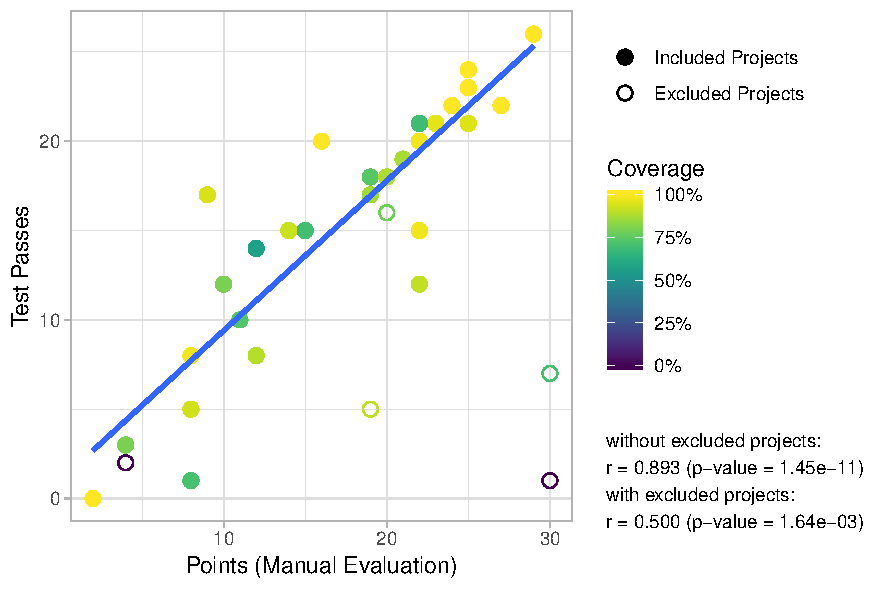
\includegraphics[width=\textwidth]{r/scatter-normal-1}
        \caption{First run}
        \label{fig:scatter_normal_1}
    \end{subfigure}%
    \begin{subfigure}{.50\textwidth}
        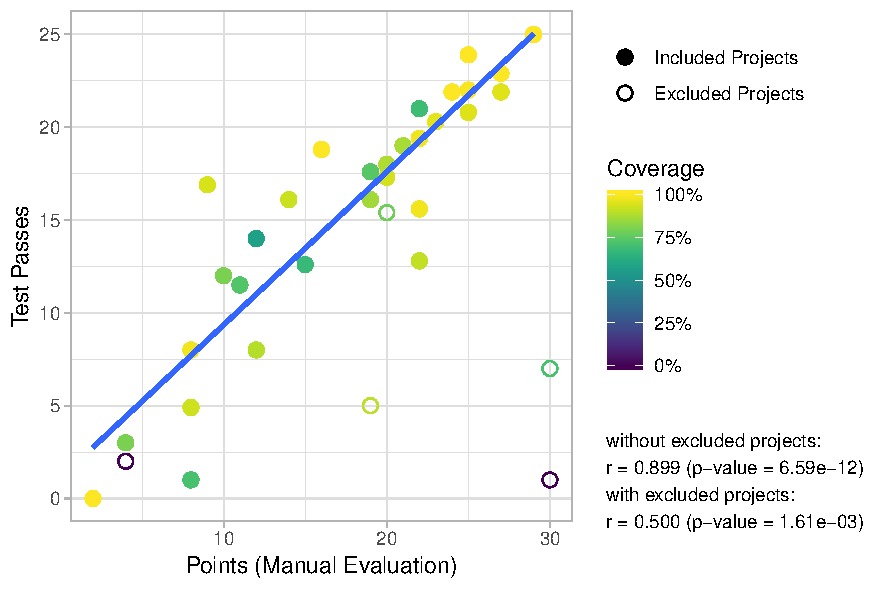
\includegraphics[width=\textwidth]{r/scatter-normal-avg}
        \caption{Average over 3 runs}
        \label{fig:scatter_normal_avg}
    \end{subfigure}
    \caption{Comparison between test results of test suite T1 (normal) and manually assigned scores}
    \label{fig:scatter_normal}
\end{figure}

\subsubsection{Input-Independent / Constraint-Only Test Suite (T2)}

Figure~\ref{fig:scatter_constraint} compares the test outcomes of test suite T2 to the manual scores.
Possible values for the number of constraint passes are in the range of $[0, 20]$.
We can, again, observe a strong correlation between the two scores,
with a correlation coefficient of $r = 0.8877$ for the first run and $r = 0.8968$ for the average over 3 runs.

\begin{figure}[htpb]
    \centering
    \begin{subfigure}{.50\textwidth}
        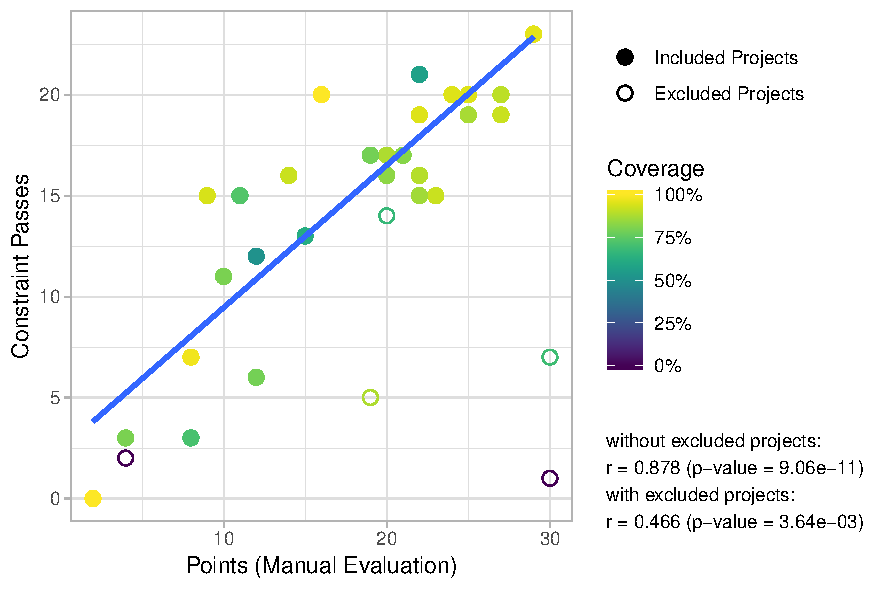
\includegraphics[width=\textwidth]{r/scatter-constraint-1}
        \caption{First run}
        \label{fig:scatter_constraint_1}
    \end{subfigure}%
    \begin{subfigure}{.50\textwidth}
        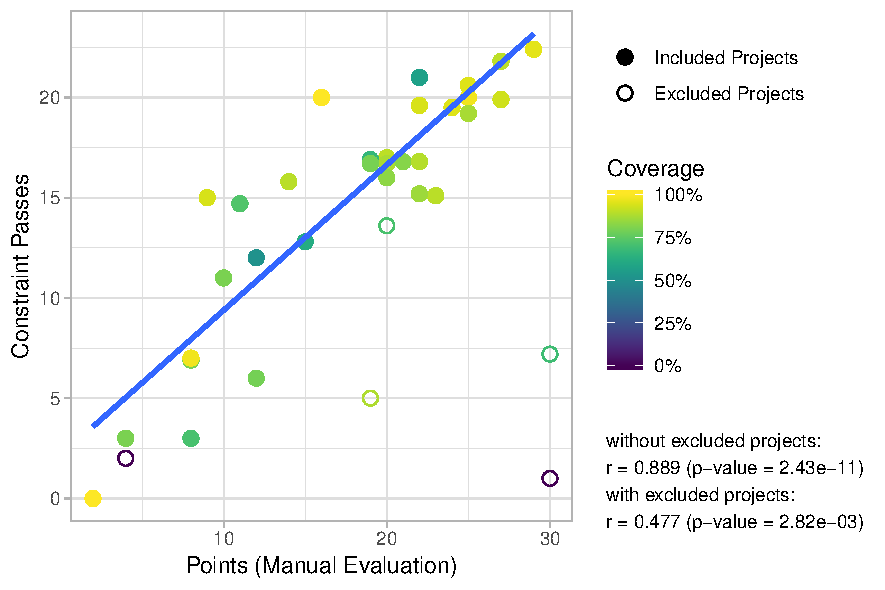
\includegraphics[width=\textwidth]{r/scatter-constraint-avg}
        \caption{Average over 3 runs}
        \label{fig:scatter_constraint_avg}
    \end{subfigure}
    \caption{Comparison between test results of test suite T2 (input-indepent / constraint-only) and manually assigned scores}
    \label{fig:scatter_constraint}
\end{figure}

\subsubsection{Random Input Test Suite (T3)}

Figure~\ref{fig:scatter_constraint} compares the test outcomes of test suite T2 to the manual scores.
Possible values for the number of constraint passes are in the range of $[0, 18]$.
The result indicate a strong correlation with a correlation coefficient of $r = 0.8629$ for the first run and $r = TODO$ for the average over 5 runs.

\begin{figure}[htpb]
    \centering
    \begin{subfigure}{.50\textwidth}
        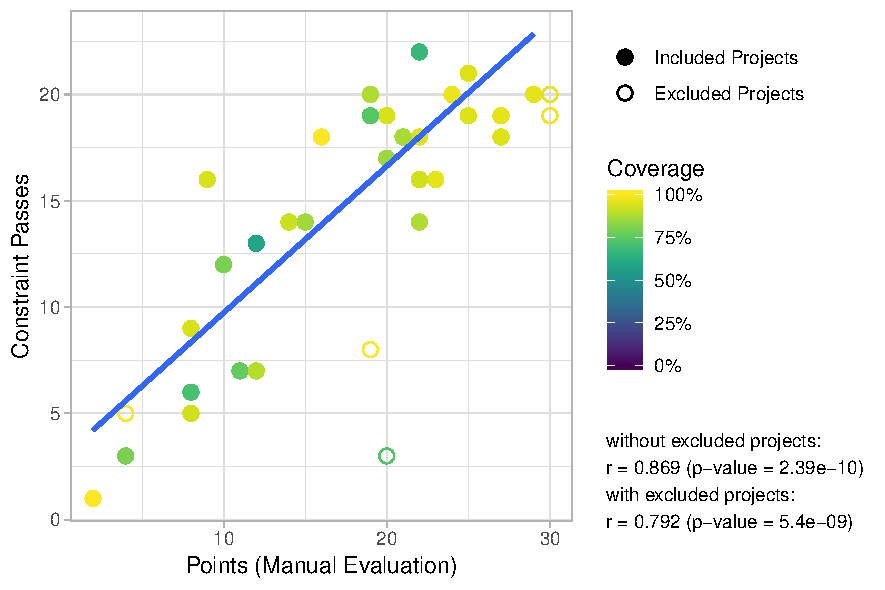
\includegraphics[width=\textwidth]{r/scatter-random-1}
        \caption{First run}
        \label{fig:scatter_random_1}
    \end{subfigure}%
    \begin{subfigure}{.50\textwidth}
        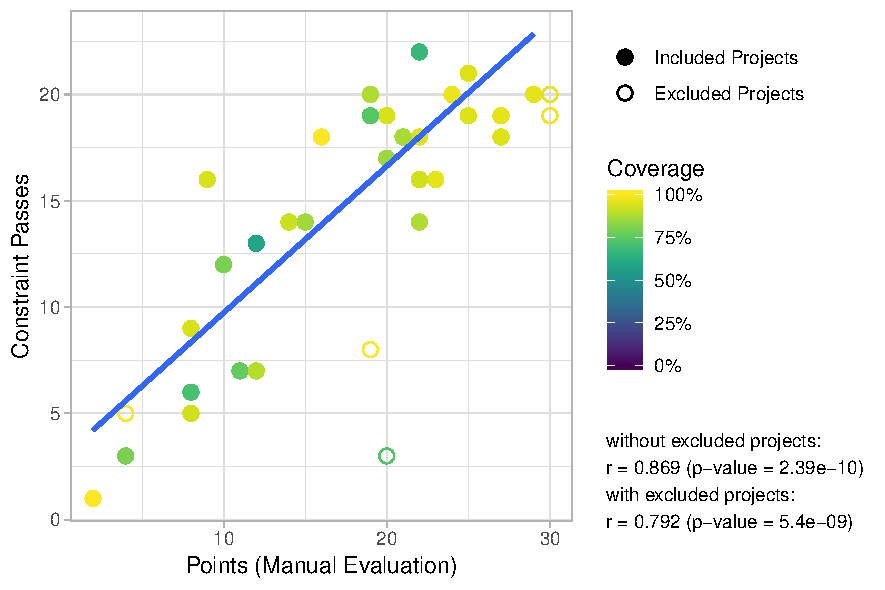
\includegraphics[width=\textwidth]{r/scatter-random-1}
        \caption{Average over 3 runs}
        \label{fig:scatter_random_avg}
    \end{subfigure}
    \caption{Comparison between test results of test suite T3 (random input) and manually assigned scores}
    \label{fig:scatter_random}
\end{figure}

\subsection{Consistency of test outcomes over multiple runs}

\paragraph{Null hypothesis ($H_0$):}
Automated test results show very different results each run and are thus not accurate enough for grading purposes.
\vspace{-\medskipamount}
\paragraph{Alternative hypothesis ($H_1$):}
Test results are consistent enough over multiple runs to provide accurate information for grading.
\parspace

In order to analyze which test cases where inconsistent for each project, and vice versa,
we construct matrices over the test cases in T1-T3, and the projects in P1.
If a test case shows inconsistent results on a certain project over five test executions,
we assign a $1$ to the respective cell in the matrix, otherwise we assign a 0.
For this, we consider both ''skipped'' and ''failed'' to be the same test outcome, since both are non-passing test results.
The matrix's sum of rows then shows us how may projects showed inconsistent test results for each test case,
and the sum of columns shows the number of test cases with inconsistent outcomes for each project.
Table~\ref{tab:inconsistencies_matrices_excerpt} shows excerpts of the resulting matrices for demonstration.
The full matrices can be found in the appendix in Section~\ref{sec:inconsistencies_matrices}.
\parspace

\begin{figure}[htpb]
    \centering

    \begin{subfigure}{.4\textwidth}
        \centering

        \setlength{\tabcolsep}{0.2em}
        \tiny
        \begin{tabular}{l|rrrrrr}
            \toprule
                    & 12         & 13         & 14         & 15         & 16         & 17         \\
            \midrule
            K6\_S02 & 0          & 0          & \textbf{1} & \textbf{1} & 0          & \textbf{1} \\
            K6\_S03 & 0          & \textbf{1} & \textbf{1} & \textbf{1} & 0          & \textbf{1} \\
            K6\_S05 & 0          & 0          & 0          & 0          & 0          & 0          \\
            K6\_S10 & 0          & \textbf{1} & \textbf{1} & 0          & 0          & 0          \\
            K6\_S11 & 0          & 0          & 0          & 0          & 0          & 0          \\
            K6\_S13 & 0          & 0          & 0          & 0          & 0          & 0          \\
            \bottomrule
        \end{tabular}
        \caption{Inconsistent test-project pairs for test suite T1}
        \label{tab:inconsistencies_matrix_excerpt_normal}
        \setlength{\tabcolsep}{\defaulttabcolsep}
    \end{subfigure}
    \vspace{.08\textwidth}
    \begin{subfigure}{.4\textwidth}
        \centering

        \setlength{\tabcolsep}{0.2em}
        \tiny
        \begin{tabular}{l|rrrrrr}
            \toprule
                    & \ 7        & \ 8        & \ 9        & 10         & 11         & 12         \\
            \midrule
            K6\_S02 & 0          & \textbf{1} & \textbf{1} & 0          & \textbf{1} & 0          \\
            K6\_S03 & 0          & 0          & 0          & 0          & 0          & 0          \\
            K6\_S05 & 0          & 0          & 0          & 0          & 0          & \textbf{1} \\
            K6\_S10 & 0          & 0          & 0          & 0          & 0          & 0          \\
            K6\_S11 & 0          & 0          & 0          & 0          & 0          & \textbf{1} \\
            K6\_S13 & 0          & 0          & 0          & 0          & 0          & 0          \\
            \bottomrule
        \end{tabular}
        \caption{Inconsistent constraint-project pairs for test suite T2}
        \label{tab:inconsistencies_matrix_excerpt_constraint}
        \setlength{\tabcolsep}{\defaulttabcolsep}
    \end{subfigure}

    \vspace{-3\bigskipamount}
    \caption{Excerpt from the test-project matrices of inconsistent test outcomes}
    \label{tab:inconsistencies_matrices_excerpt}
\end{figure}

\subsubsection{Normal Test Suite (T1)}

\mnote{Is there a threshold above which a test suite is considered too flaky}
\noindent Figure~\ref{fig:consistency_per_test_normal} shows the number of inconsistent test-project pairs per test case of T1.
The horizontal line displays the average number of inconsistencies per test case.
Figure~\ref{fig:consistency_per_project_normal} shows the number of inconsistent test-projects pairs per project.
We can observe that some test cases and some projects tend to be rather inconsistent,
with a maximum of $5$ inconsistent projects ($16.13\%$ of projects) per test case and $5$ inconsistent test cases ($17.86\%$ of test cases) per project.
However, on average only $1.06$ projects per test case and $1.18$ test cases per project show inconsistent results.
This amounts to $3.80\%$ of all test-project pairs, which is still consistent enough for grading purposes.
\parspace

\begin{figure}[htpb]
    \centering
    \begin{subfigure}{.65\textwidth}
        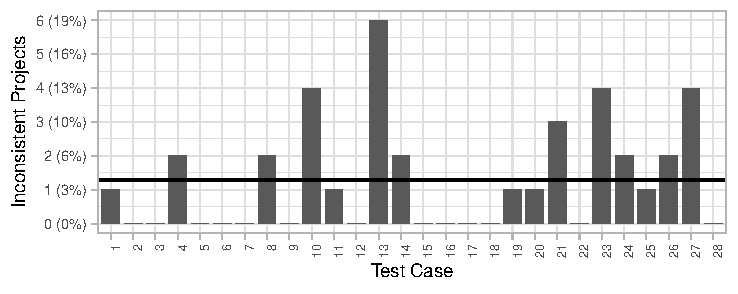
\includegraphics[width=\textwidth]{r/consistency-per-test-normal}%
        \vspace{-\medskipamount}
        \caption{Number of projects with inconsistent outcomes, per test case}
        \label{fig:consistency_per_test_normal}
    \end{subfigure}
    \begin{subfigure}{.65\textwidth}
        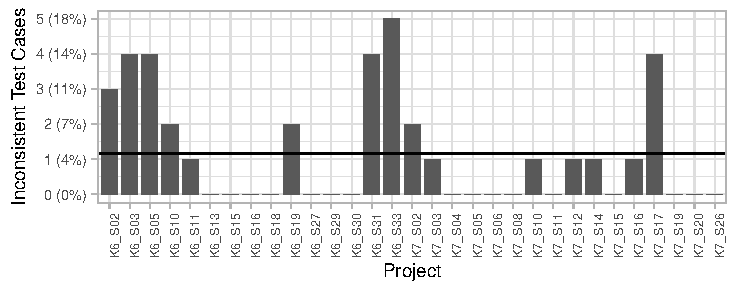
\includegraphics[width=\textwidth]{r/consistency-per-project-normal}%
        \vspace{-\medskipamount}
        \caption{Number of test cases with inconsistent outcomes, per project}
        \label{fig:consistency_per_project_normal}
    \end{subfigure}

    \caption{Inconsistent outcomes of test suite T1 over 5 runs}
    \label{fig:consistency_normal}
\end{figure}

\subsubsection{Input-Independent / Constraint-Only Test Suite (T2)}

Figure~\ref{fig:consistency_per_test_constraint} shows the number of inconsistencies for test suite T2.
We observe similar results to T1.
The data shows a maximum of $5$ inconsistent projects ($16.13\%$ of projects) per constraint and $5$ inconsistent constraints ($25.00\%$ of constraints) per project.
On average, $1.38$ projects per constraint and $0.94$ constraints per project show inconsistent results,
which amounts to $4.45\%$ of all constraint-project pairs.
\parspace

\begin{figure}[htpb]
    \centering
    \begin{subfigure}{.65\textwidth}
        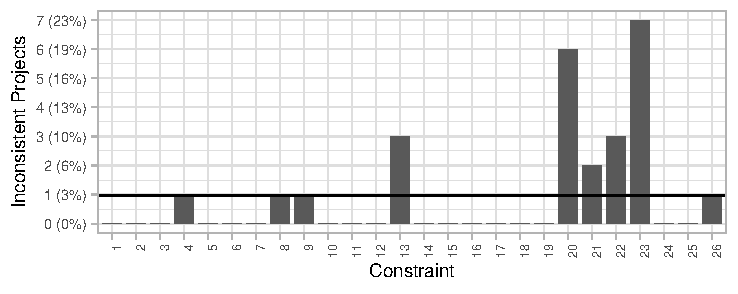
\includegraphics[width=\textwidth]{r/consistency-per-test-constraint}%
        \vspace{-\medskipamount}
        \caption{Number of projects with inconsistent outcomes, per constraint}
        \label{fig:consistency_per_test_constraint}
    \end{subfigure}
    \begin{subfigure}{.65\textwidth}
        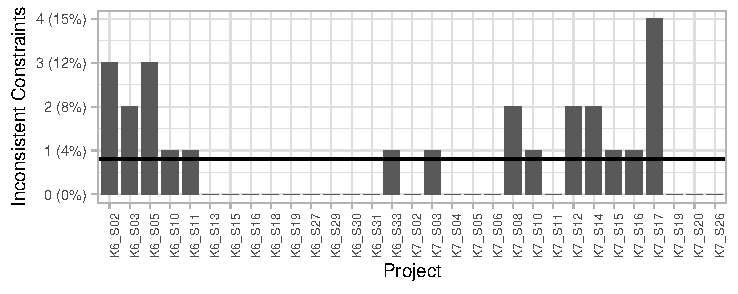
\includegraphics[width=\textwidth]{r/consistency-per-project-constraint}%
        \vspace{-\medskipamount}
        \caption{Number of constraints with inconsistent outcomes, per project}
        \label{fig:consistency_per_project_constraint}
    \end{subfigure}

    \caption{Inconsistent outcomes of test suite T2 over 5 runs}
    \label{fig:consistency_constraint}
\end{figure}

\subsubsection{Random Input Test Suite (T3)}

Figure~\ref{fig:consistency_per_test_constraint} shows the number of inconsistencies for test suite T3.
We observed a maximum of $7$ inconsistent projects ($22.58\%$ of projects) per constraint and $5$ inconsistent constraints ($27.78\%$ of constraints) per project.
On average, $2.94$ projects per constraint and $1.71$ constraints per project show inconsistent results,
which amounts to $9.58\%$ of all constraint-project pairs.
Since this test suite is non-deterministic and executes the programs longer than the other test suites,
this increase in inconsistent outcomes is expected.

\parspace

\begin{figure}[htpb]
    \centering
    \begin{subfigure}{.65\textwidth}
        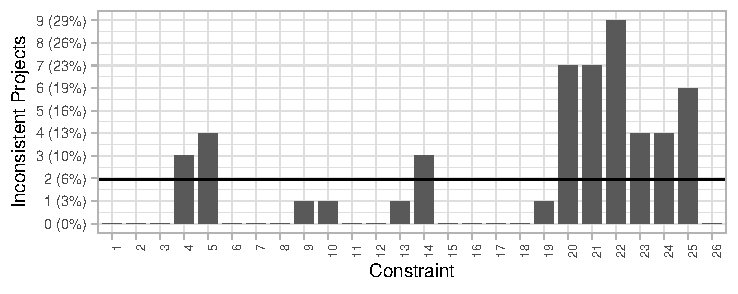
\includegraphics[width=\textwidth]{r/consistency-per-test-random}%
        \vspace{-\medskipamount}
        \caption{Number of projects with inconsistent outcomes, per constraint}
        \label{fig:consistency_per_test_random}
    \end{subfigure}
    \begin{subfigure}{.65\textwidth}
        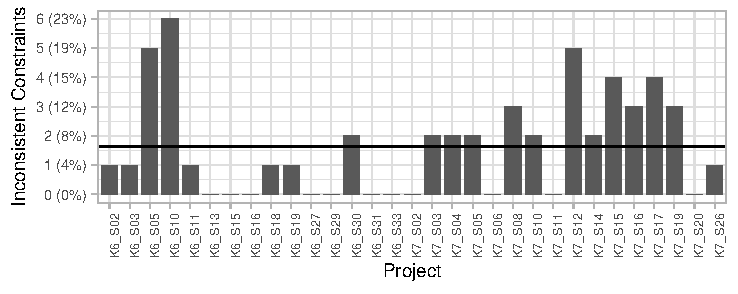
\includegraphics[width=\textwidth]{r/consistency-per-project-random}%
        \vspace{-\medskipamount}
        \caption{Number of constraints with inconsistent outcomes, per project}
        \label{fig:consistency_per_project_random}
    \end{subfigure}

    \caption{Inconsistent outcomes of test suite T3 over 5 runs}
    \label{fig:consistency_random}
\end{figure}

\subsection{Causes for inconsistent test outcomes}

\mnote{In the discussion, write that Scratch programs tend to be inconsistent / non-deterministic because of their multimedia nature}
Inconsistent test outcomes can be caused by either the test or the project under test.
Therefore, we analyzed the inconsistencies of test suite T1 and their cause in Table~\ref{tab:inconsistencies_causes_normal}.
Most of them are caused by projects behaving in a non-deterministic manner,
tough some are caused by test cases themselves.
We noticed that tests, which deal with the banana sprite, i.e. test cases $13, 14, 15, 17, 23, 24, 25$ all have a high number of inconsistent results.
We observed two reasons for this:
Firstly, the banana sprite is often poorly implemented, which causes it to be Inconsistent.
We suspect that students did not pay much attention to the banana sprite, since it is not essential to play the game.
A banana, which touches the ground, just subtracts points, while an apple, that falls to the ground, ends the game.
Secondly, tests, which deal with the banana sprite are more likely to be inconsistent.
In order to not go game over, tests have to periodically catch the falling apple with the bowl.
This means, that the tests do not always, and are not always even able to, catch bananas with the bowl,
which introduces inconsistency to tests, that rely on the behaviour of the banana.
\parspace

\begin{table}[htpb]
    \centering

    \scalebox{0.95}{
    \scriptsize
    \begin{tabular}{lrlp{11.25cm}}
        \toprule
        Project & Test & Cause   & Description \\
        \midrule
        K7\_S16 & 4    & Project & Program sometimes goes game over directly after being started. \\

        K6\_S03 & 8    & Project & Program moves banana to a random position on the ground when right arrow key is pressed.
                                   Therefore the test has different outcomes depending if the apple spawns left or right of the bowl. \\
        K6\_S33 & 8    & Both    & Test waits for 250ms to let the program initialize, then waits for a banana to appear at the top of the screen.
                                   K6\_S33 lets the banana fall instantly instead of waiting for a second (as specified),
                                   causing the banana to be below the tests threshold for detecting the banana ($y > 100$) after 250ms. \\

        K6\_S10 & 13   & Project & Program checks if the apple touches the ground with Scratch's "touching edge" primitive.
                                   Therefore, the program sometimes goes game over when an apple randomly spawns too much to the side of the screen and touches a vertical edge. \\
        K7\_S03 & 13   & Project & Program does not move banana to the top of the screen when it touches the ground, only when it touches the bowl.
                                   Therefore, the banana stays on the ground and is moved only when bowl moves over it, making banana re-spawns dependent on apple spawn locations. \\
        K7\_S07 & 13   & Project & Test checks if a certain number of bananas spawn in 30 seconds.
                                   Bananas fall very slowly in this project.
                                   Because of this, enough bananas spawn if multiple bananas are randomly caught by the bowl,
                                   but too few bananas spawn if bananas fall to the ground instead, because they have to travel more distance before they re-appear. \\

        K6\_S02 & 14   & Project & Banana get stuck in the ground and only re-spawns if touched by the bowl. \\
        K6\_S10 & 14   & Test    & Test checks if bananas spawn at random x coordinates.
                                   The program uses clones for fruit sprites.
                                   The test detects the original sprite and the clone as two banana instances at the same x coordinate concludes that bananas spawn at the same x coordinate. \\
        K7\_S12 & 14   & Test    & Test checks if bananas spawn in random positions, and failed because it detected two bananas spawning in the same position.
                                   In order to speed up test executions, we decided to wait for only two bananas to spawn and compare their positions.
                                   Therefore, while unlikely, it is possible that two bananas spawn in the same place by random chance, which fails the test. \\

        K7\_S17 & 19   & Project & Programs are supposed to check if the apple touches the color of the red stripe at the bottom to detect when the apple touches the ground.
                                   K7\_S17 checks for the wrong shade of red which is only present in some places, at the transition of the background and the red line.
                                   Therefore sprites are sometimes not detected touching the ground, and simply stay at the bottom of the screen. \\

        K6\_S05 & 20   & Project & To move the banana to a random position whenever it spawns,
                                   the program uses Scratch's builtin ''go to random position'', which moves it to a random y coordinate as well.
                                   Afterwards, it immediately adjusts the bananas y coordinate.
                                   But for a split second, the banana may touch the bowl or the ground without interaction, which the test detects. \\

        K7\_S02 & 21   & Both    & Program moves the apple to a random position on the ground 2 seconds after game over, causing the test to recognize it as not game over.
                                   The test could wait longer before performing checks to circumvent this problem. \\
        K7\_S10 & 21   & Project & Banana sometimes re-appears one more time after game over. \\
        K6\_S10 & 23   & Test    & Test relies on the banana touching the bowl, but only follows the apple with the bowl in order to not go game over.
                                   Therefore, sometimes the banana does not touch the bowl at all, resulting in a failing test. \\
        K6\_S19 & 23   & Test    & The test checks if score is added when the apple touches the bowl.
                                   It is skipped if the apple and the banana touch the bowl / ground in quick succession,
                                   because the wrong score change might be considered, or the two score changes might happen in the same step. \\

        K6\_S02 & 27   & Both    & Banana can get stuck in the ground and continually subtract points for a short time after the time is up. \\
        K6\_S19 & 27   & Both    & Banana sometimes still falls for a short time after the time is up. \\
        \bottomrule
    \end{tabular}
    }

    \medskip

    \scalebox{0.95}{
    \tiny
    \begin{tabular}{lrlp{3.875cm}|lrlp{3.875cm}}
        \toprule
        Project & Test & Cause   & Description &
        Project & Test & Cause   & Description \\
        \midrule
        K6\_S03 & 14   & Project & See K6\_S03, test 8. &
        K7\_S03 & 14   & Project & See K7\_S03, test 13. \\
        K7\_S07 & 14   & Project & See K7\_S07, test 13. &
        K6\_S02 & 15   & Project & See K6\_S02, test 14. \\
        K6\_S03 & 15   & Project & See K6\_S03, test 8. &
        K7\_S07 & 15   & Project & See K7\_S07, test 13. \\
        K6\_S02 & 17   & Project & See K6\_S02, test 14. &
        K6\_S03 & 17   & Project & See K6\_S03, test 8. \\
        K7\_S03 & 17   & Project & See K7\_S03, test 8. &
        K7\_S07 & 17   & Project & See K7\_S07, test 13. \\
        K7\_S17 & 21   & Project & See K7\_S17, test 19. &
        K6\_S05 & 23   & Project & See K6\_S05, test 20. \\
        K7\_S07 & 23   & Test    & See K6\_S10, test 23. &
        K7\_S17 & 23   & Test    & See K6\_S19, test 23. \\
        K7\_S17 & 23   & Test    & See K6\_S10, test 23. &
        K6\_S05 & 24   & Project & See K6\_S05, test 20. \\
        K7\_S15 & 24   & Test    & See K6\_S19, test 23. &
        K7\_S17 & 24   & Project & See K7\_S17, test 19. \\
        K7\_S26 & 24   & Project & See K6\_S19, test 23. &
        K6\_S05 & 25   & Project & See K6\_S05, test 20. \\
        K6\_S03 & 13   & Project & See K6\_S03, test 8. \\
        \bottomrule
    \end{tabular}
    }

    \caption{Inconsistent outcomes of test suite T1 on projects P1 and their causes}
    \label{tab:inconsistencies_causes_normal}
\end{table}

%        1 2 3 4 5 6 7 8 9 10 11 12 13 14 15 16 17 18 19 20 21 22 23 24 25 26 27
% K6_S02                                1  1     1                             1
% K6_S03               1             1  1  1     1
% K6_S05                                                  1        1  1  1
% K6_S10                             1  1                          1
% K6_S11
% K6_S13
% K6_S15
% K6_S16
% K6_S18
% K6_S19                                                           1           1
% K6_S27
% K6_S29
% K6_S30
% K6_S31
% K6_S33               1
% K7_S02                                                     1
% K7_S03                             1  1        1
% K7_S04
% K7_S05
% K7_S06
% K7_S07                             1  1  1     1                 1
% K7_S08
% K7_S10                                                     1
% K7_S11
% K7_S12                                1
% K7_S14
% K7_S15                                                              1
% K7_S16       1
% K7_S17                                               1     1     1  1
% K7_S19                                                           1
% K7_S20
% K7_S26                                                              1

\section{RQ2: Automated Input Generation}
\label{sec:rq2}

\mnote{For random tests, expect only average results to be usable, because of how the caching game works\\TODO: add the coverage ''test''}

For this part of the evaluation, we will consider following research question:

\begin{center}\begin{minipage}{.9\textwidth}
    \textbf{RQ2: Is automated test input generation a viable method to control Scratch programs for testing purposes?}
\end{minipage}\end{center}

\noindent In RQ1, we already showed, that accurate test results with random input are possible.
In order to get good test results generally, the generated input needs to be able to execute as much of the program as possible.
Intuitively, the more of a program gets executed, the more of the its functionality can be checked by tests running on it.
Therefore, we want to find out how much of a typical Scratch program's functionality can be reached by controlling it through Whisker's generated user input.
In order to measure how much of the program is reached, we will use the achieved statement coverage as an indicator.
\parspace

We ran Whisker's automated input generation algorithm on each of the Code Club Scratch projects (P2) for ten minutes,
and measured the current statement coverage every second during the execution.
We chose not to reset the programs during the execution time,
since some of Code Club's projects require much execution time to be covered.
In fact, we also tried a configuration of $4 * 2.5\text{min}$ (ten minutes with four resets)
and got worse results.
% Each program was run for five minutes and was reset five times during that time,
% resulting five one-minute executions of the program.
We use the mean final statement coverage on the projects to indicate how much of the programs is reached by the automated input.
To get more consistent results, we ran this experiment five times, and took the average of the final coverage scores.
Listing~\ref{lst:coverage_test} shows the code, which we used to run the programs.
We chose to simulate random inputs with a duration between $100\text{ms}$ and $1000\text{ms}$ in an interval of $250\text{ms}$.
In order to access the coverage during the execution we implemented a function called \texttt{logCoverage},
which saves the current statement coverage of the program and outputs all saved coverage records once the test is over.
\parspace

% \mnote{TODO: remove?}
% \textbf{Correlation of test results and manual scoring.}
% Secondly, we want to determine how accurate results from tests with automatically generated input are.
% For this purpose, we tested the catching game projects (P1) with test suites T3 and T4,
% which are variations of the input-independent test suite T2, that uses Whisker's automated input generation to control the program.
% The catching game projects are especially challenging to be tested with automated input,
% since the catching game has a game over state, which is difficult to avoid.
% Like in RQ1, we use the correlation between test results and manual scores as an indicator of the test results' quality.
% \parspace

\begin{listing}[ht]
    \centering

    \begin{minipage}{.9\textwidth}
        \begin{javascriptcode}
            const coverageTest = async function (t) {
                t.detectRandomInputs({duration: [100, 1000]});
                t.setRandomInputInterval(250);

                for (let timestamp = 1000; timestamp <= 600000; timestamp += 1000) {
                    await t.runUntil(() => t.getTotalTimeElapsed() >= timestamp);
                    t.logCoverage(timestamp, t.isProjectRunning());
                }

                t.end();
            }
        \end{javascriptcode}
    \end{minipage}

    \caption{Test case to measure the coverage of automatically generated input}
    \label{lst:coverage_test}
\end{listing}

\subsection{Coverage Measurements}

\paragraph{Null hypothesis ($H_0$):}
Automated input generation can only cover a small fraction of typical Scratch programs' code, making it infeasible for testing purposes.
Program coverage with automated input is not better than coverage without any input.
\paragraph{Alternative hypothesis ($H_1$):}
Automated input generation is able to reach most of typical Scratch programs' functionality, making it a viable method to control the Scratch programs for testing.
Program coverage with automated input is much higher than coverage without input.
\parspace

\noindent Figure~\ref{fig:coverage} shows the statement coverage, which we were able to achieve on the Code Club projects (P2)
with Whisker's automatically generated input,
as well as the execution time at which the coverage was achieved.
The black line in Figure~\ref{fig:coverage_line} displays the mean coverage of the projects over time.
After ten minutes of run time, we were able to achieve an average coverage of $95.25\%$ with the lowest coverage for a project being $74\%$ and the highest being $100\%$.
We repeated this experiment five times and got similar results, with the mean final coverage over five runs being $TODO\%$.
In comparison, Figure~\ref{fig:coverage_no_input} shows the achieved coverage without simulating any inputs.
Here, we only got an average of $47.04\%$ per project on our first run, and $TODO\%$ averaged over five runs.
\parspace

\begin{figure}[htpb]
    \centering
    \begin{subfigure}{.8\textwidth}
        \includegraphics[width=\textwidth]{r/coverage-bar-run-1}
        \caption{Coverage per project}
        \label{fig:coverage_bar}
    \end{subfigure}
    \begin{subfigure}{.8\textwidth}
        \includegraphics[width=\textwidth]{r/coverage-line-run-1}
        \caption{Coverage over time}
        \label{fig:coverage_line}
    \end{subfigure}

    \caption{Achieved coverage with automated input}
    \label{fig:coverage}
\end{figure}

\begin{figure}[htpb]
    \centering
    \begin{subfigure}{.8\textwidth}
        \includegraphics[width=\textwidth]{r/coverage-bar-no-input-run-1}
        \caption{Coverage per project}
        \label{fig:coverage_no_input_bar}
    \end{subfigure}
    \begin{subfigure}{.8\textwidth}
        \includegraphics[width=\textwidth]{r/coverage-line-no-input-run-1}
        \caption{Coverage over time}
        \label{fig:coverage_no_input_line}
    \end{subfigure}

    \caption{Achieved coverage without input}
    \label{fig:coverage_no_input}
\end{figure}

\subsection{Reasons for low coverage on certain projects}

Over the five runs with generated input, we observed ''Create Your Own World'' and ''Memory'' to consistently have the lowest coverage of the projects.
% A screenshot of both these programs can be seen in Figure~\ref{fig:difficult_code_club_projects}.
We are going to take a quick look at the reasons, why these projects are difficult to cover by using random input.

\begin{itemize}
    \item ''Create Your Own World'' implements a little adventure game with a player sprite, which starts on the left of the screen and is able to move through several rooms through a portal on the right side of the screen.
        This project is difficult to cover, because the sprite needs to move a long way in one direction, to reach a screen transition.
        But because each arrow key has equal probability to be simulated by Whisker, the sprite will likely only hover over a small area around its start position.
    \item In ''Memory'' the player can hit 4 different colored drums.
        The player has to hit them in an order, which is randomly determined by the program.
        If the player hits one drum incorrectly, which includes hitting a drum while no sequence is active, the game goes into a game over state,
        and can only be restarted by pressing the green flag.
        Therefore, using random inputs quickly results in an irrecoverable game over,
        because a wrong drum is hit, which renders much of the program's code unreachable.
\end{itemize}

% \begin{figure}[htpb]
%     \centering
%
%     \begin{subfigure}{.3\textwidth}
%         \centering
%         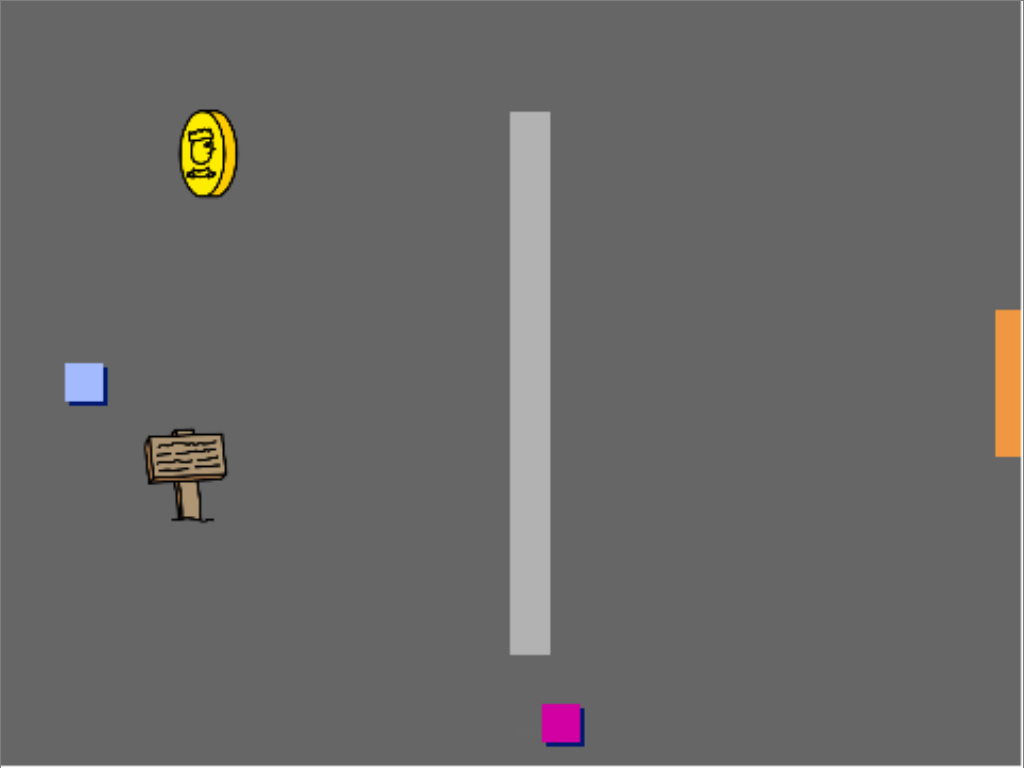
\includegraphics[width=\textwidth]{code-club-create-your-own-world}
%         \caption{Create Your Own World}
%     \end{subfigure}
%     \hspace{1mm}
%     \begin{subfigure}{.3\textwidth}
%         \centering
%         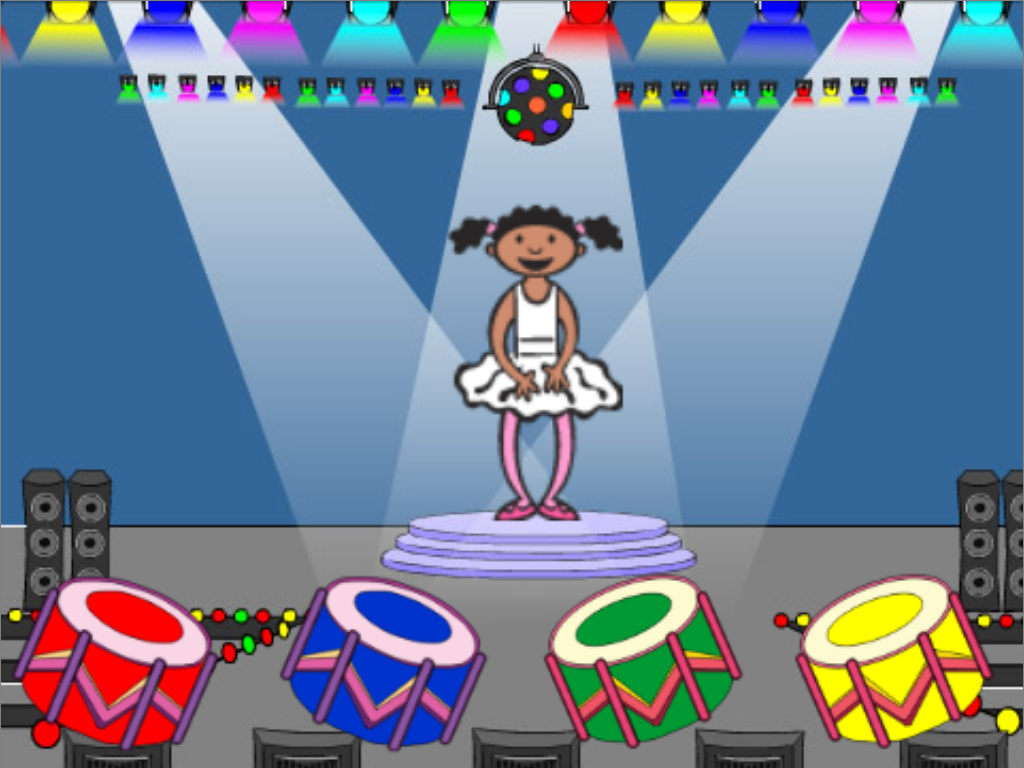
\includegraphics[width=\textwidth]{code-club-memory}
%         \caption{Memory}
%     \end{subfigure}%
%
%     \caption{Difficult to cover Code Club projects}
%     \label{fig:difficult_code_club_projects}
% \end{figure}

\section{RQ3: Interference with Programs Under Test}
\label{sec:rq3}

In the following section, we want to answer another research question:

\begin{center}\begin{minipage}{.9\textwidth}
    \textbf{RQ3: Does the testing process slow down the program under test?}
\end{minipage}\end{center}

\noindent Since JavaScript is executed in a single-threaded environment,
Whisker executing code in between steps of the Scratch program can possibly be problematic.
Additional computations could take too long and delay the next step of the program.
Scratch offers blocks which delay the execution of a script for a set amount of time.
These blocks save the current time when called and wait until a certain time difference between the current time and the saved time is reached.
Therefore, if the program is executed too slowly, fewer blocks are executed while the delay is active,
which can make a difference if the program expects to get a certain amount of work done during the wait.
However, we suspect that this will not be a concern for most Scratch programs.
\parspace

Scratch's step function has to be called 30 times per second.
Therefore, the execution time of Whisker's step function, which includes the execution of Scratch's step function,
should not exceed $1000\text{ms}/30 = 33.33\text{ms}$.
Scratch allocates $0.75 * 33.33\text{ms} = 25.0\text{ms}$ of the $33.33\text{ms}$ to execute the program.
If no sprite changes in the program during the step,
the Scratch VM will execute the program for the allocated amount of time.
But if some sprite's position or appearance changes, the VM will stop executing the program earlier.
Afterwards, Scratch draws the new frame in the GUI.
In the worst case, i.e. if no sprite changes and the whole time interval is used to execute the program,
$0.25 * 33.33\text{ms} = 8.33\text{ms}$ will be left to render the new frame.
Most modern hardware will take less time than $8.33\text{ms}$ to render the picture,
which leaves time for Whisker to execute other tasks.
\parspace

We should also note that some of Whisker's optional functionality gets executed during Scratch's step,
which will slow the program down as well, if the full $25\text{ms}$ of execution time are used by Scratch.
This includes coverage measurement and callbacks for sprite changes (e.g. \texttt{t.onSpriteMoved} and \texttt{spite.onMoved}).
However the Scratch GUI itself also registers code to update the GUI, which is run during the step of the VM,
so this should not affect the program, unless the registered callbacks are very expensive to execute.
\parspace

To evaluate this, we measured the execution time of Whisker's components (see Figure~\ref{fig:whisker_step_procedure})
as well as the execution time of Scratch during each step.
Since we execute Whisker in a web browser,
we were limited to JavaScript's \texttt{performance.now} method to measure execution times.
\texttt{performance.now} returns the time, since which the current web page is open,
with an accuracy of $0.1\text{ms}$.
The code we used for measuring the execution times can be found in Listing~\ref{lst:time_measurement_code} in the appendix.
\parspace

We executed our test suites T1-T3 on the sample solution of the catching game (P1) ten times,
and measured the execution times.
We will consider the mean times, as well as the maximum times from the ten runs
to decide if the test execution could interfere with the program or not.

\subsection{Time measurements}

\paragraph{Null hypothesis ($H_0$):}
The execution of additional code delays the execution of Scratch's steps, which possibly interferes with the program execution.
\vspace{-\medskipamount}
\paragraph{Alternative hypothesis ($H_1$):}
The execution of additional code introduces no delay. It will therefore not interfere with the program execution.
\parspace

Figure \ref{fig:time_line_plot} shows execution times from the first run of each test suite on the program.
It displays the total execution time of Whisker's step procedure over time.
The time measurements include both the execution time of Whisker and Scratch.
We can see that the execution time is mostly far beneath the limit of $33.33\text{ms}$
and only rarely spikes to higher for short periods of time.
\parspace

\begin{figure}[htpb]
    \centering

    \begin{subfigure}{\textwidth}
        \centering
        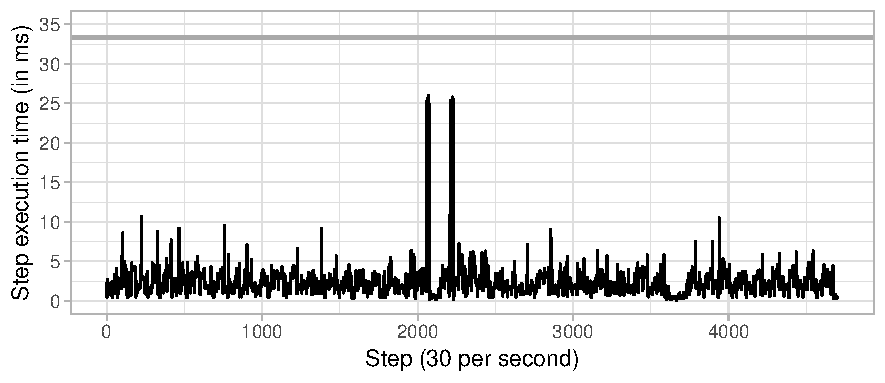
\includegraphics[width=.7\textwidth]{r/time-normal}
        \vspace{-\medskipamount}
        \caption{T1 (normal)}
    \end{subfigure}

    \begin{subfigure}{\textwidth}
        \centering
        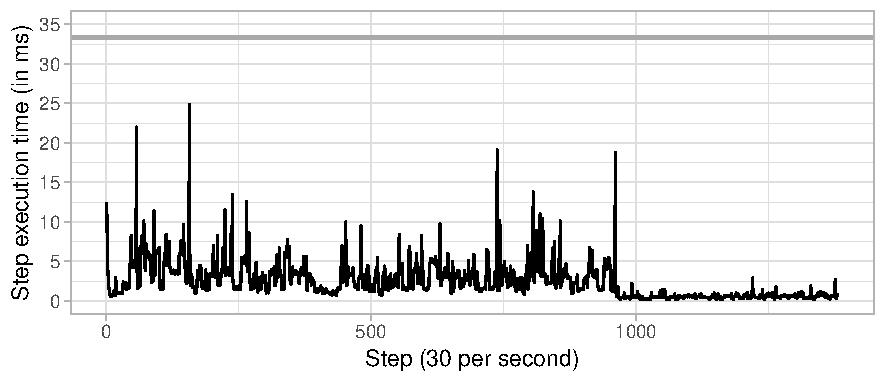
\includegraphics[width=.7\textwidth]{r/time-constraint}
        \vspace{-\medskipamount}
        \caption{T2 (input-independent / constraint-only)}
    \end{subfigure}

    \begin{subfigure}{\textwidth}
        \centering
        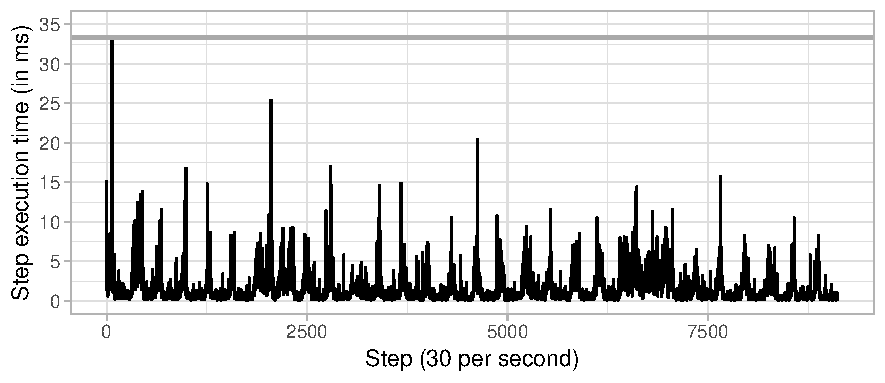
\includegraphics[width=.7\textwidth]{r/time-random}
        \vspace{-\medskipamount}
        \caption{T3 (random input)}
    \end{subfigure}

    \caption{Measured execution time of Whisker's step procedure during first test execution}
    \label{fig:time_line_plot}
\end{figure}

Figure \ref{tab:time_measurements} shows the mean and maximum of executions times for each part of Whisker's step procedure.
This data is taken from ten consecutive executions of the respective test suite on the program under test.
Again, the average total execution time is far beneath $33.33\text{ms}$.
The execution of test suite T1 spiked over the $33.33\text{ms}$ with a maximum of $35.1\text{ms}$,
but this only happened in one step, with the second longest step execution time for T1 being $31.1\text{ms}$.

% round((0.071 + 0.102 + 0.068) / 3, digits = 3)
% round((0.004 + 0.004 + 0.024) / 3, digits = 3)
% round((0.005 + 0.005 + 0.023) / 3, digits = 3)
% round((0.022 + 0.022 + 0.022) / 3, digits = 3)
% round((1.852 + 2.054 + 1.129) / 3, digits = 3)
% round((0.007 + 0.006 + 0.005) / 3, digits = 3)
% round((0.012 + 0.078 + 0.058) / 3, digits = 3)
% round((1.972 + 2.272 + 1.330) / 3, digits = 3)
% round((0.12  + 0.218 + 0.201) / 3, digits = 3)
%
% round(max(4.8  , 7.3  , 9.7 ), digits=3)
% round(max(1.3  , 3.1  , 6.4 ), digits=3)
% round(max(2    , 1.6  , 8.6 ), digits=3)
% round(max(6.4  , 4.2  , 4.8 ), digits=3)
% round(max(35.1 , 24.6 , 32.7), digits=3)
% round(max(1.1  , 0.3  , 1.8 ), digits=3)
% round(max(2.9  , 3.2  , 12.5), digits=3)
% round(max(35.1 , 24.9 , 33.1), digits=3)
% round(max(6.5  , 7.6  , 13.1), digits=3)

\begin{table}[htpb]
    \centering
    \footnotesize
    \begin{tabular}{l|rr|rr|rr}
        \toprule
                             &       & T1   &       & T2   &       & T3   \\
                             & mean  & max  & mean  & max  & mean  & max  \\
        \midrule
        Callbacks (Before)   & 0.071 & 4.8  & 0.102 & 7.3  & 0.068 & 9.7  \\
        Random Inputs        & 0.004 & 1.3  & 0.004 & 3.1  & 0.024 & 6.4  \\
        Inputs               & 0.005 & 2    & 0.005 & 1.6  & 0.023 & 8.6  \\
        Sprites              & 0.022 & 6.4  & 0.022 & 4.2  & 0.022 & 4.8  \\
        Scratch              & 1.852 & 35.1 & 2.054 & 24.6 & 1.129 & 32.7 \\
        Callbacks (After)    & 0.007 & 1.1  & 0.006 & 0.3  & 0.005 & 1.8  \\
        Constraints          & 0.012 & 2.9  & 0.078 & 3.2  & 0.058 & 12.5 \\
        \midrule
        Total                & 1.972 & 35.1 & 2.272 & 24.9 & 1.330 & 33.1 \\
        Total (Whisker only) & 0.12  & 6.5  & 0.218 & 7.6  & 0.201 & 13.1 \\
        \bottomrule
    \end{tabular}
    \caption{Measured execution time (in ms) for every part of Whisker's step procedure}
    \label{tab:time_measurements}
\end{table}

{\Huge redo this on the laptop for external validity}

\section{Discussion}
\label{sec:discussion}

In this evaluation, we conducted three separate experiments to prove the usefulness of Whisker.
\parspace

In the first experiment, we analyzed test results of three different test suites and compared them to a ground truth.
We found out, that all of the results consistently show a strong correlation to the ground truth.
Therefore, the null hypothesis is rejected.
We proved, that the input-independent / constraint-only testing approach can deliver accurate test results,
both with deliberate input and with generated input.
Then, we analyzed the flakiness of the test suites and found several reasons,
why certain tests and certain programs can be inconsistent.
We measured the average number of these inconsistencies,
and found it low enough to reject the null hypothesis.
We suspect that simpler programs can be tested with much fewer inconsistencies.
At the same time, more experience in automated testing for Scratch will lead to more robust and less flaky test suites.
The test suites we used were written pretty early in development.
\parspace

The second experiment dealt with automated input generation.
We let Whisker's automated input generation algorithm run on several Scratch programs,
then we ran the same programs without any input.
We compared measured the statement coverage we achieved on the programs during both runs,
and compared their averages.
Since the coverage with automated input was much higher that coverage without input,
we rejected the null hypothesis.
\parspace

Aside from the research questions, we conducted another experiment to find out,
if the testing process interferes with the program under test.
For this purpose, we measured the execution time of Whisker's step procedure on the execution of our test suites
to find out if it slowed down the Scratch program.
We found out that Scratch's allocated time interval for computations is large enough to
allow executing both the Scratch program and test code.
Programs under test are not affected by Whisker, therefore, we can reject the null hypothesis.



For the generated random input, we reset the program under test 30 times and let it run for a total of $30 * 10\text{s} = 300\text{s}$.
Of course, other configurations are possible.
We chose this configuration, because the program under test will go game over in the first ten seconds most of the time.
- other configurations of time * iterations possible for random tests and coverage measurement
- execution times can be forced to be high, but aren't for normal programs / tests

\section{Threats to Validity}
\label{sec:threats_to_validity}

As is usual, the empirical studies we conducted in this work must confront certain threats to validity.
Possible threats fall into one of two categories.
On the one hand, threats to internal validity represent factors which provide alternative explanations for the presented results.
On the other hand, threats to external validity deal with the generalizability of our approach.

\subsection{Internal validity}

Conditions, which could influence any test outcomes, coverage measurements,
or time measurements are possible threads to internal validity.
\parspace

\textbf{Independence of ground truth.}
One threat to validity arises from our use of the manual scores as
ground truth to assess the quality of test results.
If we assigned the scores ourselves,
a comparison to them would not be adequate to give evidence about the quality of results.
\mnote{TODO: name}
However, the manual scores were assigned by TODO after the course was held,
before work on Whisker was even started.
Therefore, the manual scores are completely independent from our test results,
and a comparison between the two is adequate.
\parspace

\textbf{Randomness.}
Another threat is, of course, random chance.
Many scratch programs use randomness, which can make test outcomes inconsistent.
To eliminate the possibility of random chance affecting our test results as much as possible, we executed each test suite ten times,
and considered the average results in addition to results from single executions.
\parspace

\textbf{RAM usage.}
% Another possible threat comes from the execution order of the programs.
One more possible threat comes from an issue of Scratch itself.
At the time of the evaluation, Scratch had a problem of consuming increasing amounts of RAM when loading many programs in succession,
which, in theory, could have interfered with the execution of our test suites.
However, we payed close attention to the RAM usage of the machine, which executed the tests.
We also performed some of our test suite executions on all projects sequentially,
and some on one half of the programs, then later on the other half.
We observed similar results with both methods, therefore this issue did not have any impact on our test results.
% This could be problematic if we executed the programs in order of descending manual scores.
% However, we executed each test suite on the projects in alphabetical order,
% and the manual scores actually show a weak positive correlation ($r = 0.43$) to the indexes of the execution order,
% meaning that the alphabetical order is closer to the order of ascending manual scores.

\subsection{External Validity}

Any factors which limit the generalizability of the results in this work are threats to external validity.
\parspace

\textbf{Programs under test.} For one thing, the program under test could be chosen poorly,
making the results not applicable for other Scratch programs.
Therefore, we tried to choose programs that are representative of Whisker's target usage in the field of education.
To evaluate the test results we chose Scratch projects from an actual Scratch course for students.
The program has user interaction, uses randomness, and has a game over state,
which are all important challenges for testing Scratch programs.
To evaluate the automated input generation,
we again went with programs from Scratch courses.
The programs feature many different input methods and interactions,
which make them suitable to evaluate automated input on.
\parspace

\textbf{Test subjects for time measurements.}
To find out if Whisker would slow down programs under test,
we executed our test suites and measured the execution times of Whisker's step procedure.
One could argue that the execution times can be raised by a variety factors.
More, as well as more computationally expensive, callbacks and constraints can be registered.
More random inputs and inputs can be registered.
And a Scratch program with more sprites can be chosen.
Therefore, tests suites can interfere with the program under tests, if they do it purposefully.
However, we wanted to measure the execution time of a realistic test suite on a realistic program.
This setup did not slow the program down,
and the measurements indicate that more expensive test suites (e.g. with a factor of x10) will still be fine as well.
\parspace

\textbf{Hardware for time measurements.}
Since the measurements of step execution times depend on the used hardware,
it is important to use a realistic testing environment for that purpose.
Therefore, we did not only perform measurements on the main computer we used for other experiments,
but also on a less powerful laptop, which we suspect is a more realistic hardware configuration for Whisker.
